\documentclass[margin=1mm]{standalone}
\usepackage[utf8]{inputenc}
\usepackage{amsmath}
\usepackage{amsfonts}
\usepackage{amssymb, bm}
\usepackage{tikz}
\usetikzlibrary{calc,arrows,positioning,shapes,shapes.gates.logic.US,trees, backgrounds}
\usetikzlibrary{fit, positioning}

\begin{document}
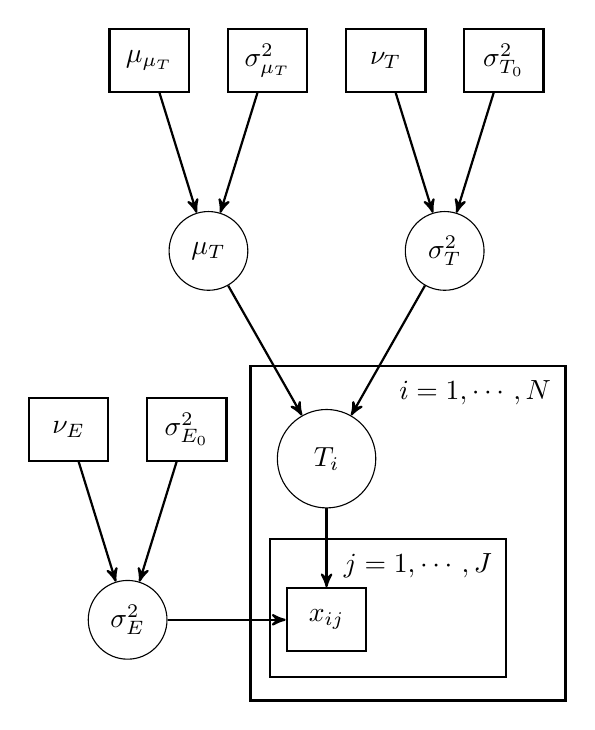
\begin{tikzpicture}[auto,scale=3,
	latent/.style={circle,draw,text badly centered, inner sep=2pt,minimum size=12.5mm},
	error/.style={circle,draw,text badly centered, inner sep=2pt,minimum size=10mm},
	manifest/.style={text centered, rectangle,draw,thick,inner sep=3pt,minimum height=8mm, minimum width=8mm, text width= 8 mm},
	  plate/.style={draw, shape=rectangle,thick, minimum height=4.25cm, minimum width=4cm, text width=1cm, align=right, inner sep=10pt, inner ysep=10pt, append after command={node[below left= 3pt of \tikzlastnode.north east] {#1}}},
	  plate2/.style={draw, shape=rectangle,thick, minimum height=1.75cm, minimum width=3cm, text width=1cm, align=right, inner sep=5pt, inner ysep=8pt, append after command={node[below left= 3pt of \tikzlastnode.north east] {#1}}},
	manifestRot/.style={text centered, rectangle, draw, thick,inner sep=3pt, minimum width=7mm, text width= 7mm, minimum height=15},
	manifestfront/.style={rectangle,draw,thick,inner sep=0pt,minimum size=12mm, fill=white},
	ghost/.style={rectangle, inner sep=0pt,text centered,    minimum height=0mm, minimum width=5mm, text width= 5 mm},
	lcorr/.style={<->,>=stealth', bend right=40},
	rcorr/.style={<->,>=stealth', bend left=40},
	fcorr/.style={<->,>=stealth', bend left=40},
	ofcorr/.style={<->,>=stealth', bend right=60},
	ofcorr2/.style={<->,>=stealth', bend left=60},
	intercept/.style={regular polygon,
        regular polygon sides=3,draw,thick,inner sep=0pt,minimum size=10mm},
	mean/.style={regular polygon,regular polygon sides=3,draw,thick,inner sep=0pt,minimum size=10mm},
	paths/.style={->, thick, >=stealth'},
	variance/.style={<->, thick, >=stealth', bend left=270, looseness=2},
	varianceTop/.style={<->, thick, >=stealth', bend right=270, looseness=2},
	unique/.style={<->, thick, >=stealth', loop below=270, looseness=8},
	factvar/.style={<->, thick, >=stealth', loop right=270, looseness=8}
	] % End Creating Path Model Pieces
\tikzset{mystyle/.style={->,double=black}}


% person model
\node [manifest] at (0,0) (x) {$x_{ij}$};
\node [latent]     [above = 1cm of x] (t) {$T_i$};
\node [error]      [above = 1.5cm of t,  xshift=-1.5cm] (mt)   {$\mu_T$};
  \node [manifest] [above = 1.5cm of mt, xshift=-.75cm] (mtp1) {$\mu_{\mu_T}$};
  \node [manifest] [above = 1.5cm of mt, xshift= .75cm] (mtp2) {$\sigma^2_{\mu_T}$};
\node [error]      [above = 1.5cm of t,  xshift= 1.5cm] (st)   {$\sigma^2_T$};
  \node [manifest] [above = 1.5cm of st, xshift=-.75cm] (stp1) {$\nu_T$};
  \node [manifest] [above = 1.5cm of st, xshift= .75cm] (stp2) {$\sigma^2_{T_0}$};
\node [error]      [left = 1.5cm of x] (se) {$\sigma^2_E$};
  \node [manifest] [above = 1.5cm of se, xshift=-.75cm] (sep1) {$\nu_E$};
  \node [manifest] [above = 1.5cm of se, xshift= .75cm] (sep2) {$\sigma^2_{E_0}$};

\node [plate={$i=1, \cdots, N$}] [right= -1.5cm of x, yshift=1.1cm] (p) {};
\node [plate2={$j=1, \cdots, J$}] [right= -1.25cm of x, yshift=0.15cm] (p2) {};


% paths
\draw[paths] (t)  -- (x);
\draw[paths] (mt) -- (t);
\draw[paths] (st) -- (t);
\draw[paths] (se) -- (x);
\draw[paths] (mtp1) -- (mt);
\draw[paths] (mtp2) -- (mt);
\draw[paths] (stp1) -- (st);
\draw[paths] (stp2) -- (st);
\draw[paths] (sep1) -- (se);
\draw[paths] (sep2) -- (se);
\end{tikzpicture}
\end{document}